\documentclass{article}

\usepackage{graphicx}
\usepackage{tikz}
\usepackage{tikzsymbols}
\usetikzlibrary{calc,patterns,shapes.geometric}
\pagestyle{empty}
\usepackage[margin=0pt]{geometry}
\geometry{papersize={14in,12in}}

\def\centerarc[#1](#2)(#3:#4:#5){\draw[#1] ($(#2)+({#5*cos(#3)},{#5*sin(#3)})$) arc (#3:#4:#5);}

\begin{document}
	\begin{figure}
		\centering
		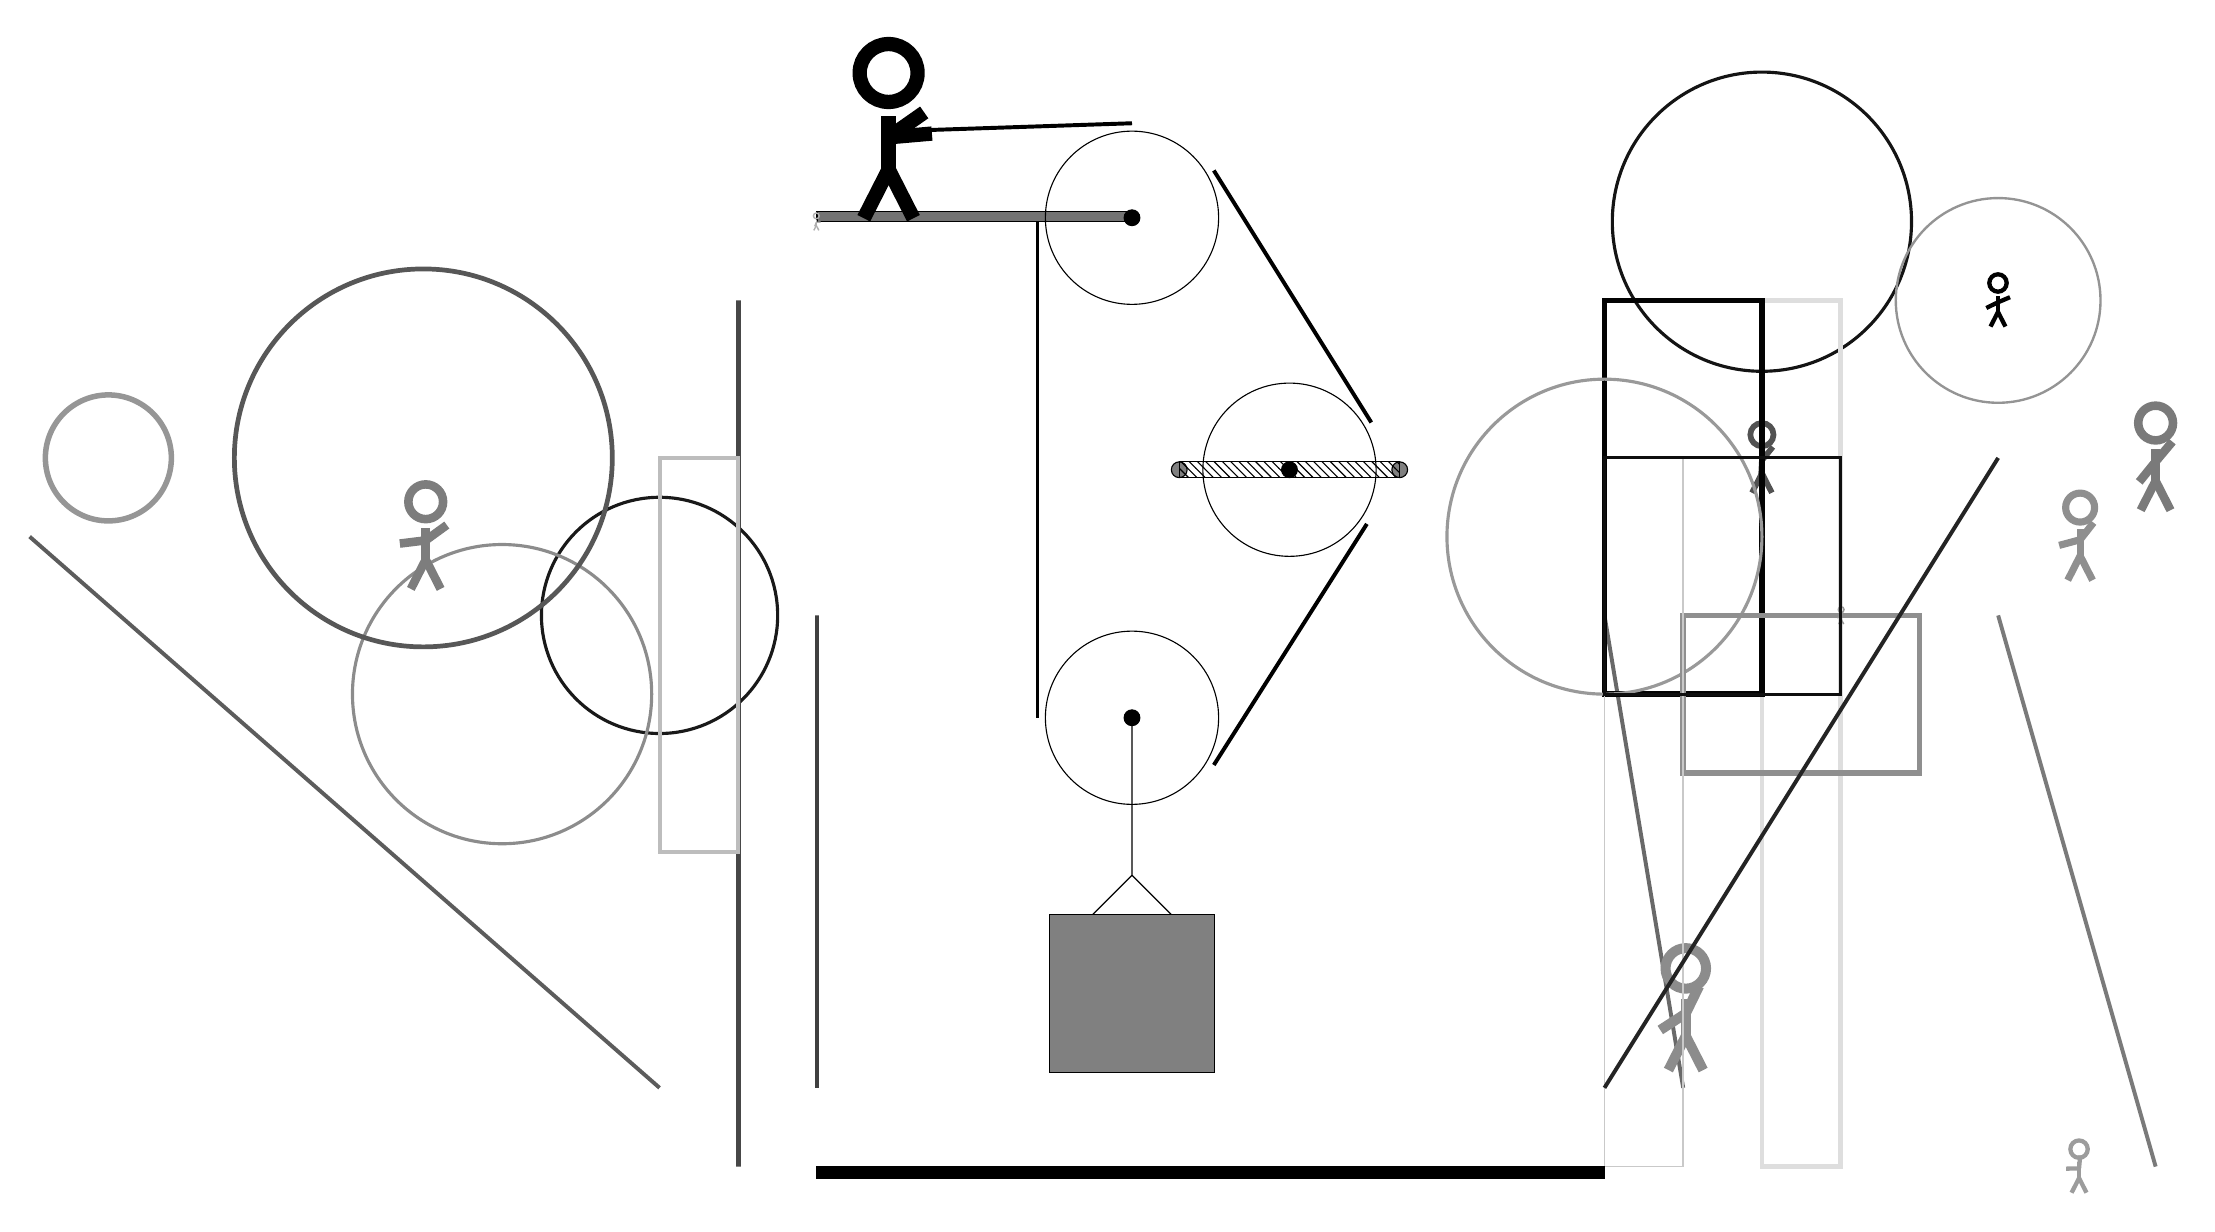
\begin{tikzpicture}
			%%%%% START %%%%%
			
			\draw[fill=black!55] (-2, 9) rectangle (2, 9.125);
			
			\draw (2, 2.7) circle (1.1);
			\draw[fill=black] (2, 2.7) circle (0.1);
			
			\draw (2, 9.05) circle (1.1);
			\draw[fill=black] (2, 9.05) circle (0.1);
			
			\draw[fill=white](4, 5.85) circle (1.1);
			\draw[fill=black] (4, 5.85) circle (0.1);
			\draw[fill=black!50] (2.6, 5.85) circle (0.1);
			\draw[fill=black!50] (5.4, 5.85) circle (0.1);
			\draw[pattern=north west lines, pattern color=black] (2.6, 5.95) rectangle (5.4, 5.75);
			
			\draw (2, 2.7) -- (2, 0.7) -- (1.5, 0.2) -- (2.5, 0.2) -- (2, 0.7);
			\draw[fill=black!50] (0.95, 0.2) rectangle (3.05, -1.8);
			
			\draw[line width=0.5mm] (0.8, 9) -- (0.8, 2.7);
			\centerarc[line width=0.5mm](2, 2.7)(180:330:1.2000000000000002);
			\draw[line width=0.5mm](3.0392, 2.1) -- (4.983, 5.1617);
			\centerarc[line width=0.5mm](4, 5.85)(390:325:1.2000000000000002);
			\draw[line width=0.5mm](5.0392, 6.45) -- (3.0392, 9.65);
			\centerarc[line width=0.5mm](2, 9.05)(30:90:1.2000000000000002);
			\draw[line width=0.5mm](2, 10.25) -- (-1, 10.15);
			
			\node at (-1, 10.15) {\Strichmaxerl[10][-175][35]};
			
			\draw [line width=0.4mm, color=black!92](10, 9) circle (1.9);
			
			\draw[line width=0.5mm, color=black!59](8, 4) -- (9, -2);
			\node[line width=0.7mm, color=black!31] at (-2, 9) {\Strichmaxerl[1][69][3]};
			\node[line width=0.4mm, color=black!68] at (10, 6) {\Strichmaxerl[4][87][51]};
			\draw[line width=0.6mm, color=black!13] (10, -3) rectangle (11, 8);
			
			\draw[line width=0.6mm, color=black!75] (-2, 4) rectangle (-2, -2);
			
			\draw [line width=0.4mm, color=black!90](-4, 4) circle (1.5);
			\draw [line width=0.4mm, color=black!45](-6, 3) circle (1.9);
			\node[line width=0.3mm, color=black!51] at (-7, 5) {\Strichmaxerl[6][7][36]};
			\draw [line width=0.3mm, color=black!42](13, 8) circle (1.3);
			
			\draw[line width=0.7mm, color=black!72] (-3, 8) rectangle (-3, -3);
			\draw[line width=0.7mm, color=black!99] (10, 3) rectangle (8, 8);
			\node[line width=0.7mm, color=black!44] at (14, 5) {\Strichmaxerl[5][15][52]};
			
			\draw [line width=0.4mm, color=black!40](8, 5) circle (2.0);
			\draw [line width=0.6mm, color=black!66](-7, 6) circle (2.4);
			\draw[line width=0.5mm, color=black!26] (-4, 1) rectangle (-3, 6);
			
			\draw[line width=0.7mm, color=black!44] (9, 2) rectangle (12, 4);
			\draw[line width=0.5mm, color=black!52](13, 4) -- (15, -3);
			\node[line width=0.6mm, color=black!52] at (15, 6) {\Strichmaxerl[6][51][50]};
			\node[line width=0.2mm, color=black!39] at (14, -3) {\Strichmaxerl[3][1][85]};
			\draw [line width=0.7mm, color=black!41](-11, 6) circle (0.8);
			
			\node[line width=0.3mm, color=black!41] at (11, 4) {\Strichmaxerl[1][26][68]};
			
			\node[line width=0.3mm, color=black!45] at (9, -1) {\Strichmaxerl[7][33][64]};
			\node[line width=0.2mm, color=black!100] at (13, 8) {\Strichmaxerl[3][26][23]};
			\draw[line width=0.2mm, color=black!21] (8, -3) rectangle (9, 6);
			
			\draw[line width=0.5mm, color=black!86](13, 6) -- (8, -2);
			\draw[line width=0.4mm, color=black!94] (8, 3) rectangle (11, 6);
			\draw[line width=0.5mm, color=black!64](-4, -2) -- (-12, 5);
			
			
			\draw[fill=black] (-2, -3) rectangle (8, -3.15);
			
			%%%%% END %%%%%
		\end{tikzpicture}
	\end{figure}	
\end{document}